\documentclass[__main__.tex]{subfiles}

\begin{document}
\paragraph{Э-02}

Рассмотрите электромагнитные волны в пространстве, свободном от зарядов и токов. Покажите, что вектора $\vec{k}$ (волновой вектор), $\vec{E}$, $\vec{B}$ образуют правую тройку в некоторой инерциальной системе отсчёта. Объясните, почему в любой другой инерциальной системе отсчёта этот факт, будучи сформулированным для преобразованных векторов, будет также иметь место.\\

Вектор $k = \frac{\omega}{V} n$, где $n$ - единичный вектор распространения волны, $V$ - скорость распространения волны, называется \textbf{волновым вектором}.

Процесс распространения электромагнитного поля в пространстве называется электромагнитной волной. Если в точке $A$ создано электрическое поле $E_1$, убывающее со временем, это соответствует появлению тока смещения, направленного к точке А, и возникновению перпендикулярно к току вихревого магнитного поля $B_1$. Магнитное поле убывает вследствие отсутствия поддерживающих его токов. Убывающее магнитное поле порождает вихревое электрическое поле $E_2$ в пространстве в "контуре" $l$. Направление $E_2$ подчиняется правилу Ленца (Индукционный ток всегда имеет такое направление, что он ослабляет действие причины, возбуждающей этот ток). Поле $E_2$ убывает, порождается магнитное поле $B_2$ и т.д. Электромагнитная волна распространяется со скоростью $V$ вдоль оси $z$ (см. Рисунок 79). Таким образом:

1) Электромагнитная волна поперечна, колебания векторов $E$ и $B$ проходят перпендикулярно направлению распространения волны (см. Рисунок 80)

2) Электрическое и магнитное поля в бегущей волне изменяются в одной фазе

3) Вектора $E$,$B$ и $V$ (а вместе с ним и $k$) в бегущей электромагнитной волне образуют так называемую правую тройку векторов.

\begin{center}
	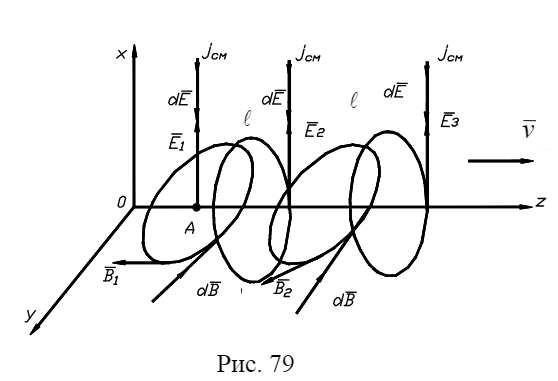
\includegraphics[]{e02_1.png}
\end{center}

\begin{center}
	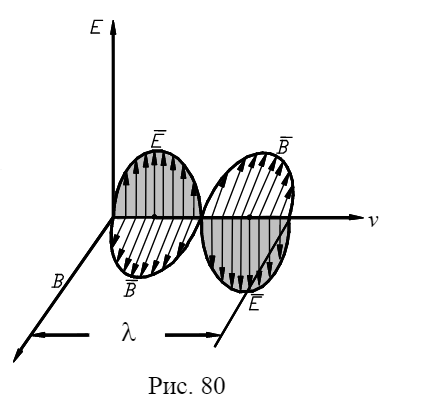
\includegraphics[]{e02_2.png}
\end{center}
\end{document}